\section{Further Details on Empirical Setup}
\label{sec:exp-details}

In this appendix we collect the additional information needed to reproduce the experiments in \cref{sec:experiments}: training data, models, optimizer hyperparameters, per-experiment grids, hardware and compute, evaluation protocol, and the supplementary figures referenced from the body.

\paragraph{Training data.} We use \texttt{smol-smoltalk} \citep{smoltalk} as our default fine-tuning corpus, using the fixed train/validation split prepared for these experiments and packing examples to sequence length $1280$. Some supplementary sweeps use \texttt{tulu-3} \citep{lambert2024tulu} with the same supervised fine-tuning pipeline. For pretraining, we train GPT-2-124M on \texttt{FineWeb} \citep{penedo2024fineweb}.

\paragraph{Models.} \cref{tab:models} summarises the five model families we consider. The fine-tuning models are initialized from the official Hugging Face checkpoints. SmolLM2 and Gemma3 use their native tokenizers.

\begin{table}[t]
\centering
\caption{Per-run training budgets. Fine-tuning runs are one epoch unless noted; pretraining uses $2.5$B-tokens.}
\small
\begin{tabular}{lrlcc}
\toprule
Model & Params & Tokenizer & Seq.\ len & Eff.\ batch / steps \\
\midrule
SmolLM2-135M       & 135M  & SmolLM2          & 1280 & 128 / 889    \\
SmolLM2-1.7B       & 1.7B  & SmolLM2          & 1280 & 256 / 1{,}778 \\
Qwen3-1.7B         & 1.7B  & Qwen BPE         & 1280 & 256 / 1{,}779 \\
Gemma3-1B          & 1.0B  & Gemma3           & 1280 & 256 / 1{,}779 \\
GPT-2-124M         & 124M  & GPT-2 BPE        & 1024 & 512 / 4{,}750 \\
\bottomrule
\end{tabular}

\vspace{2pt}
\footnotesize The SmolLM2-135M method-comparison pool used in Fig.~\ref{fig:bema_sf} uses a long-budget rerun with 3{,}557 steps.

\label{tab:models}
\end{table}

\paragraph{Training.} Unless stated otherwise for the Schedule-Free and WSD baselines, AdamW-family runs use the standard defaults $(\beta_1, \beta_2) = (0.9, 0.999)$, $\varepsilon = 10^{-8}$, weight decay $\omega = 10^{-2}$, gradient clipping at $1.0$, and a $50$-step linear warmup followed by a constant learning rate (no decay). Training uses $\texttt{bfloat16}$ mixed precision. When needed, we use gradient accumulation to reach the reported effective batch size. Headline runs use seed $42$. The learning rate $\eta$ varies per experiment and is reported in \cref{tab:hp_per_experiment}.

\paragraph{Optimizer hyperparameters.} \pace\ adds three tunable hyperparameters on top of standard AdamW: the pullback strength $c$, the EMA power $\kappa$, and the update frequency $\mathrm{uf}$ (per-experiment values in \cref{tab:hp_per_experiment}). We use $\gamma=1.0$, $\rho=0$, and clamp the per-parameter (per-coordinate) pullback gain $\lambda_{t,i}$ at $1$, matching the implementation defaults. For Schedule-Free \citep{defazio2024schedule} we use the authors' reference implementation under their published NanoGPT recipe ($\beta_1{=}0.98$, $\beta_2{=}0.95$, weight decay $0.05$, no gradient clipping); learning rate is matched per model.

\begin{table}[h]
\centering
\caption{Sweep space used by the body and appendix figures.}
\footnotesize
\renewcommand{\arraystretch}{1.15}
\setlength{\tabcolsep}{5pt}
\begin{tabular}{@{}l l p{0.53\textwidth}@{}}
\toprule
\textbf{Figures} & \textbf{Cell} & \textbf{Sweep space} \\
\midrule
\ref{fig:train_curves}, \ref{fig:c_kappa}, \ref{fig:appendix_full_train_curves}
  & 1B fine-tuning
  & SmolLM2-1.7B: $\eta\!\in\!\{3,7,10\}{\times}10^{-4}$\newline
    Qwen3-1.7B: $\eta\!\in\!\{3,5\}{\times}10^{-4}$\newline
    Gemma3-1B: $\eta\!\in\!\{10^{-3},5{\times}10^{-3}\}$\newline
    Plotted $c$ bins $\in\!\{10^{-4},5{\times}10^{-4},10^{-3},3{\times}10^{-3},$\newline
    $\phantom{\text{Plotted }c\text{ bins }\in\!\{}10^{-2},3{\times}10^{-2},10^{-1},3{\times}10^{-1}\}$\newline
    $\kappa\!\in\!\{0.2,0.5,0.7\}$, $\mathrm{uf}{=}1$
  \\
\midrule
\ref{fig:appendix_tulu_qwen}
  & Qwen3-1.7B Tulu
  & $\eta\!\in\!\{3,5\}{\times}10^{-4}$, $\kappa\!\in\!\{0.2,0.5,0.7\}$\newline
    $c\!\in\!\{5{\times}10^{-2},10^{-1},1.5{\times}10^{-1},2.5{\times}10^{-1}\}$
  \\
\midrule
\ref{fig:clip_frac_body}, \ref{fig:appendix_clip_frac}, \ref{fig:appendix_clip_frac_vs_c}
  & SmolLM2-1.7B clipping
  & Same SmolLM2-1.7B fine-tuning runs as above; clipping telemetry is reported for $\eta\!\in\!\{3{\times}10^{-4},10^{-3}\}$, $\kappa\!\in\!\{0.2,0.5,0.7\}$, and $c\!\in\!\{5{\times}10^{-3},1.5{\times}10^{-2},5{\times}10^{-2},1.5{\times}10^{-1},5{\times}10^{-1}\}$.
  \\
\midrule
\ref{fig:135m_grid}, \ref{fig:appendix_135m_full_grid}
  & SmolLM2-135M
  & Dense sweep: $\eta\!\in\!\{1,\;1.5,\;2,\;3,\;5\}{\times}10^{-3}$\newline
    $c\!\in\!\{0,\;10^{-4},\;10^{-3},\;3{\times}10^{-3},\;10^{-2},$\newline
    $\phantom{c\!\in\!\{}3{\times}10^{-2},\;10^{-1},\;3{\times}10^{-1}\}$\newline
    $\kappa\!\in\!\{0.3,\,0.5,\,0.7\}$, $\mathrm{uf}\!\in\!\{1,\,5,\,10\}$
  \\
\midrule
\ref{fig:bema_sf}, \ref{fig:appendix_train_curves}, \ref{fig:appendix_wsd_val_curves}, \ref{fig:appendix_wsd_finetune}
  & Method and WSD comparisons
  & SmolLM2-135M: AdamW/EMA/\pace\ at $\eta\!\in\!\{10^{-3},5{\times}10^{-3}\}$;\newline
    Schedule-Free: $\eta\!\in\!\{10^{-3},\;3{\times}10^{-3},\;5{\times}10^{-3},\;10^{-2}\}$\newline
    WSD baselines use $\eta\!\in\!\{1,1.5,2,3,5\}{\times}10^{-3}$\newline
    Qwen3-1.7B: AdamW/EMA/\pace\ at $\eta\!\in\!\{3,5\}{\times}10^{-4}$; Schedule-Free at $\eta\!\in\!\{3{\times}10^{-4},10^{-3}\}$.
  \\
\midrule
\ref{fig:pretrain}, \ref{fig:appendix_pretrain_kappa_sweep}, \ref{fig:appendix_pretrain_csweep}
  & GPT-2-124M
  & $\eta\!\in\!\{3{\times}10^{-4},\; 10^{-3},\; 1.5{\times}10^{-3},\; 2{\times}10^{-3},$\newline
    $\phantom{\eta\!\in\!\{}2.5{\times}10^{-3},\; 3{\times}10^{-3},\; 10^{-2}\}$\newline
    $c$: coarse grid $10^{-4}$--$3{\times}10^{-1}$ plus local grid $1{\times}10^{-3}$--$10^{-2}$\newline
    $\kappa\!\in\!\{0.2,\,0.5,\,0.7\}$, $\mathrm{uf}{=}1$
  \\
\midrule
\ref{fig:appendix_fig1_all_schedules}, \ref{fig:appendix_multiseed_robust}
  & 1B schedules and seeds
  & Schedules $\in\!\{$constant, cosine, WSD$\}$ for AdamW/\ema\ at each model's headline $\eta$ ($10^{-3}$ for SmolLM2-1.7B and Gemma3-1B, $5{\times}10^{-4}$ for Qwen3-1.7B); \pace\ at a constant $\eta$.\newline
    Multi-seed: SmolLM2-1.7B at $\eta{=}10^{-3}$, seeds $\{42,1337,2024\}$.
  \\
\midrule
\ref{fig:bema_sf}
  & SmolLM2-135M budgets
  & AdamW WSD at token budgets $\{444,667,889\}$ steps,\newline
    $\eta\!\in\!\{3,5\}{\times}10^{-3}$; \pace\ at a constant learning rate over the full budget ($c{=}10^{-1}$, $\kappa{=}0.3$).
  \\
\midrule
\ref{fig:pretrain}, \ref{fig:appendix_pretrain_csweep}, \ref{fig:appendix_pretrain_csweep_kappa}
  & GPT-2-124M schedules
  & Shared grid per schedule (constant, cosine, WSD) at $\eta{=}2{\times}10^{-3}$:\newline
    $c\!\in\!\{3{\times}10^{-4},10^{-3},2{\times}10^{-3},3{\times}10^{-3},5{\times}10^{-3},7{\times}10^{-3},10^{-2}\}$\newline
    $\kappa\!\in\!\{0.1,0.2,0.3,0.5\}$, plus AdamW and \ema, each trained at three seeds $\{0,1,42\}$.
  \\
\midrule
\ref{fig:appendix_pretrain_river}
  & GPT-2-124M budgets
  & WSD at token budgets $\{2375,3563,4750\}$ steps\newline
    ($\eta{=}2{\times}10^{-3}$, $\kappa{=}0.5$, $c{=}3{\times}10^{-3}$); the token-budget overlay uses \pace\ at a constant learning rate ($c{=}2{\times}10^{-3}$, $\kappa{=}0.5$).
  \\
\bottomrule
\end{tabular}

\label{tab:hp_per_experiment}
\end{table}

\paragraph{Hardware and compute.} Fine-tuning runs used NVIDIA RTX PRO 6000 Blackwell (98\,GB) cards; the GPT-2 pretraining sweep used Google Cloud TPU v6e (Trillium) chips. Per-run budgets are listed in \cref{tab:models}.

\paragraph{Evaluation.} For supervised fine-tuning we report held-out cross-entropy on the fixed validation split for each dataset. For pretraining we report cross-entropy on a fixed FineWeb validation shard. EMA-family methods are evaluated using $\theta_t^{\mathrm{EMA}}$ rather than the live iterate (we swap weights at evaluation time and restore them afterwards); plain AdamW reports its live-weight value; Schedule-Free reports its native vanilla evaluation since SF does not maintain a separate estimator.

\paragraph{Reproducibility.} We will release the code and configuration files needed to reproduce the reported sweeps.

\subsection{Supplementary figures}
\label{sec:exp-details-figs}

This subsection collects the full hyperparameter-sweep and figures
referenced from \cref{sec:experiments} and the result appendices; takeaways are
stated in the captions and discussed where each figure is cited.

\begin{figure}[t]
  \centering
  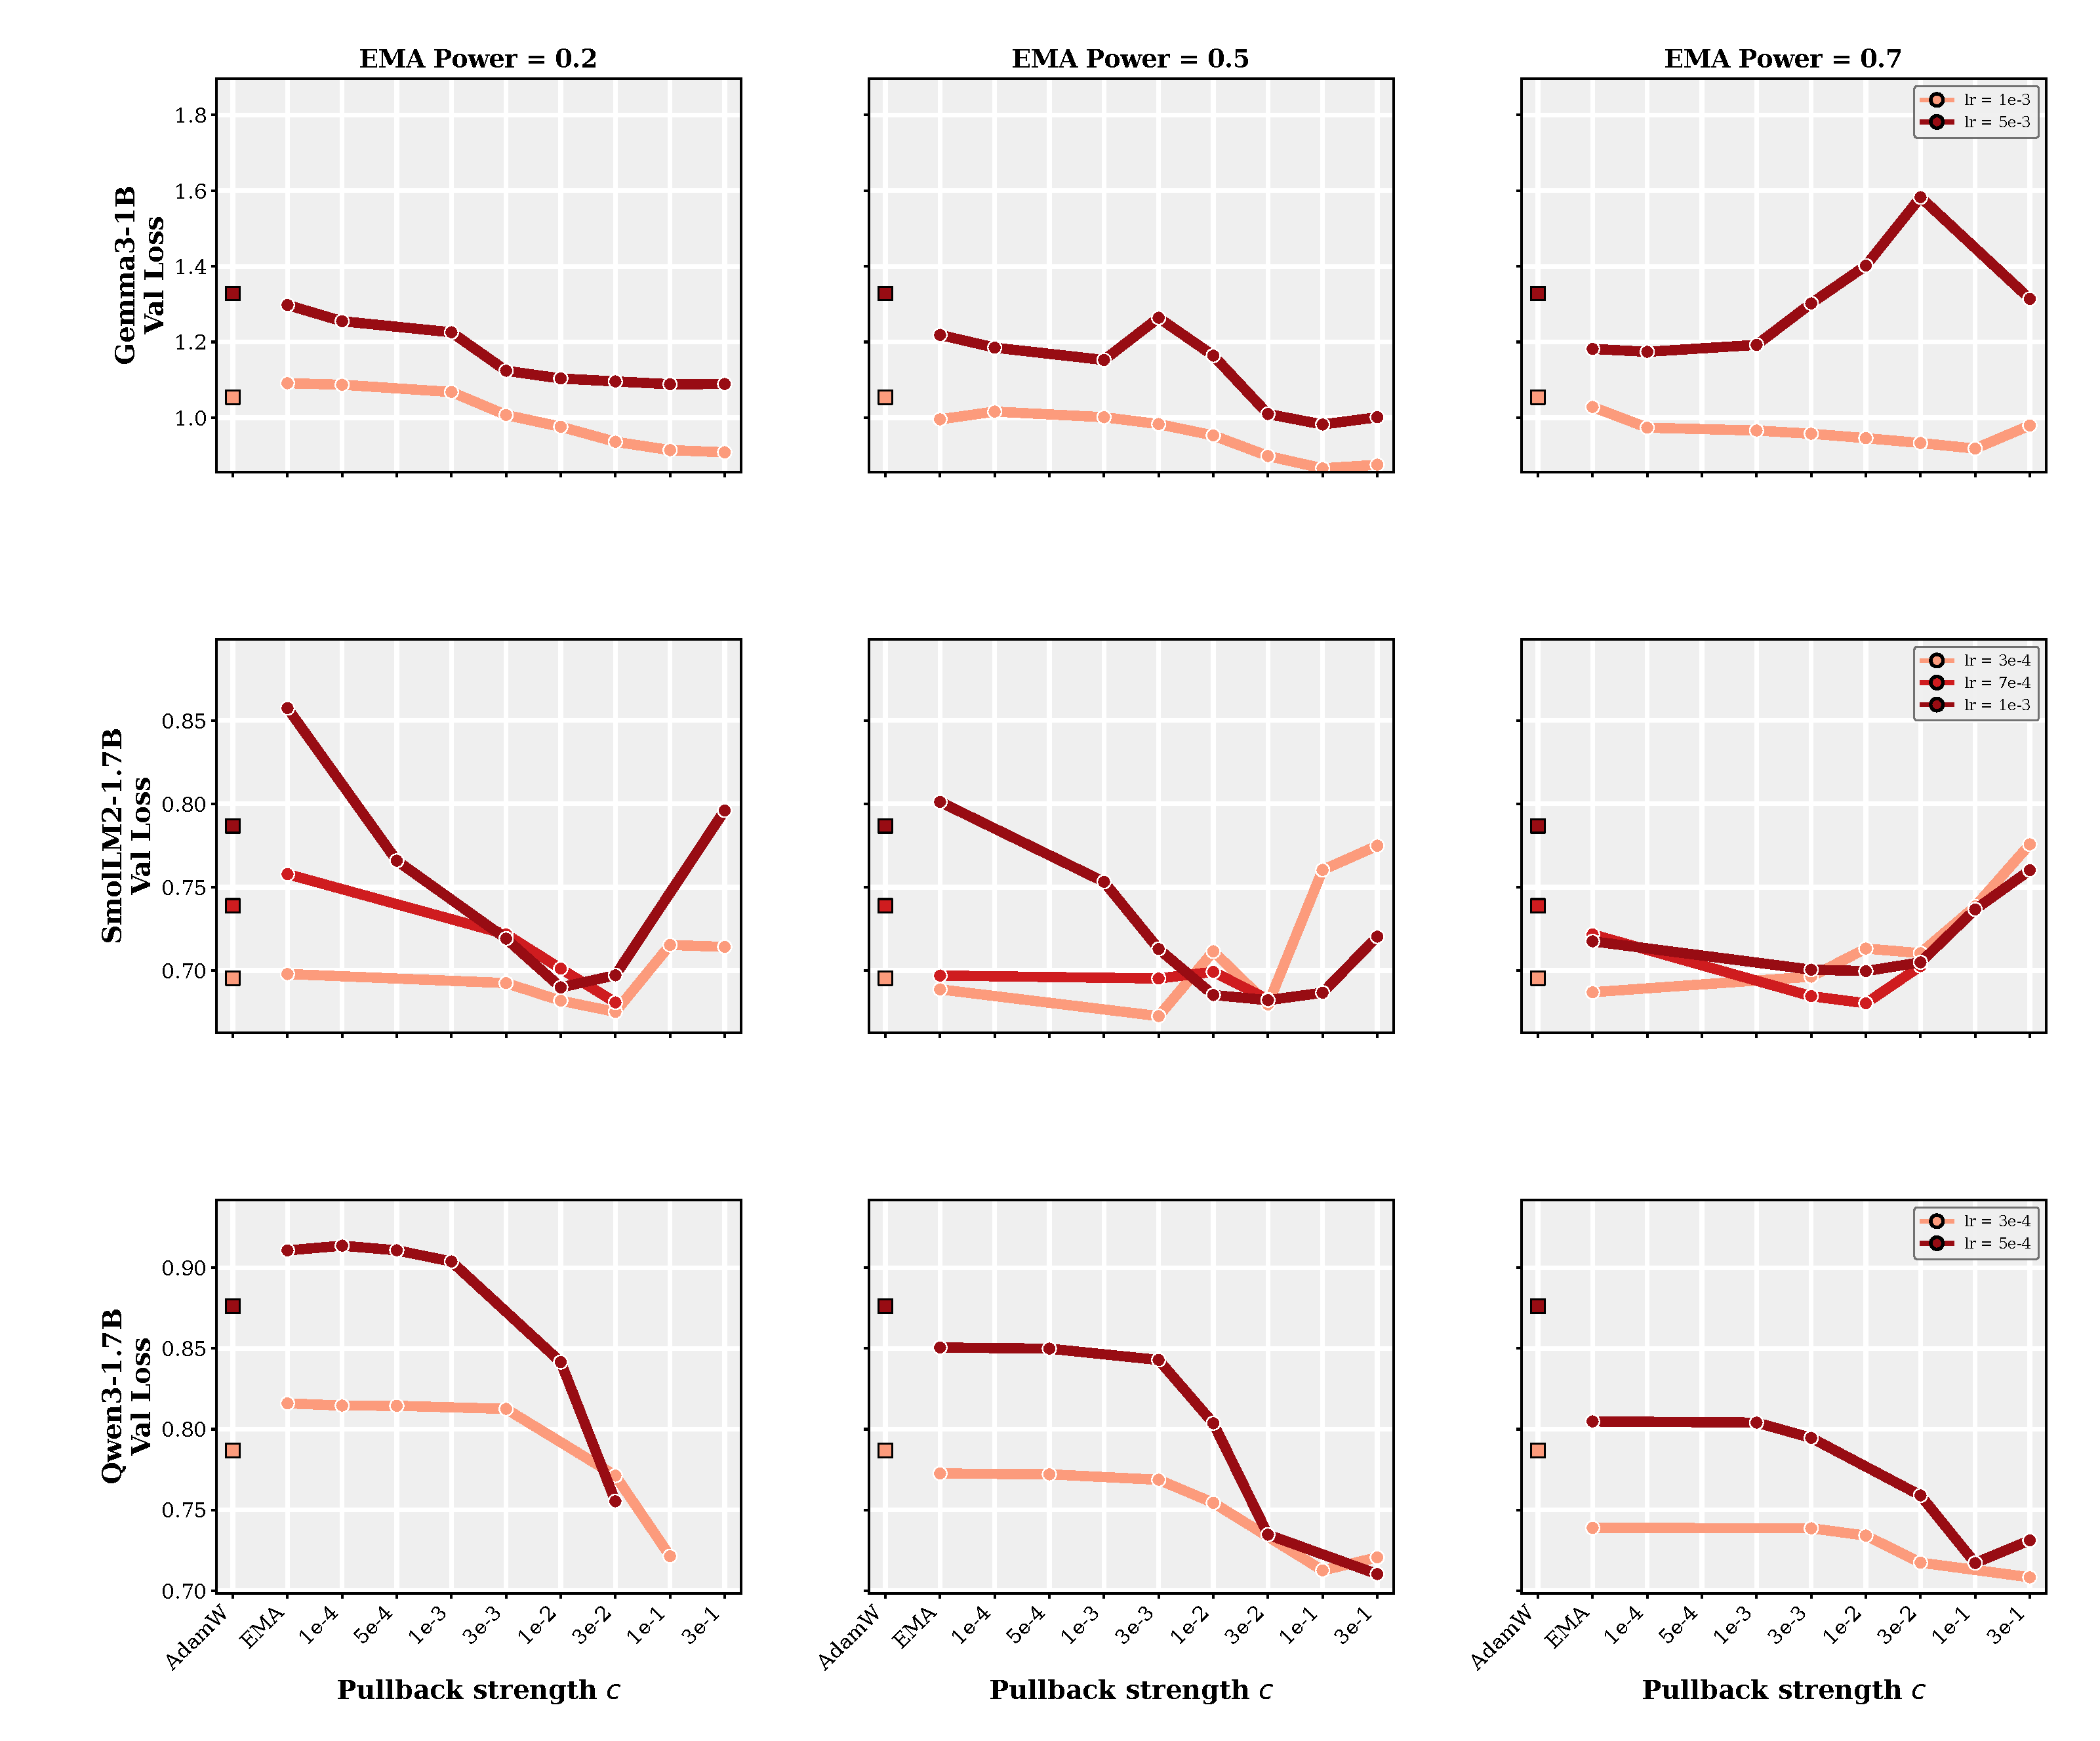
\includegraphics[width=\textwidth]{figures/fig_appendix_c_kappa_all_models.pdf}
  \captionof{figure}{\textbf{Effect of EMA power and pullback strength on SmolLM2-1.7B, Qwen3-1.7B, and Gemma3-1B.} Validation cross-entropy across learning rates, pullback strengths, and EMA powers. Optimal pullback strength remains relatively robust to learning rate and EMA power, with improvement over the EMA baseline across a wide range of settings and models.}
  \label{fig:c_kappa}
\end{figure}

\begin{figure}[ht]
  \centering
  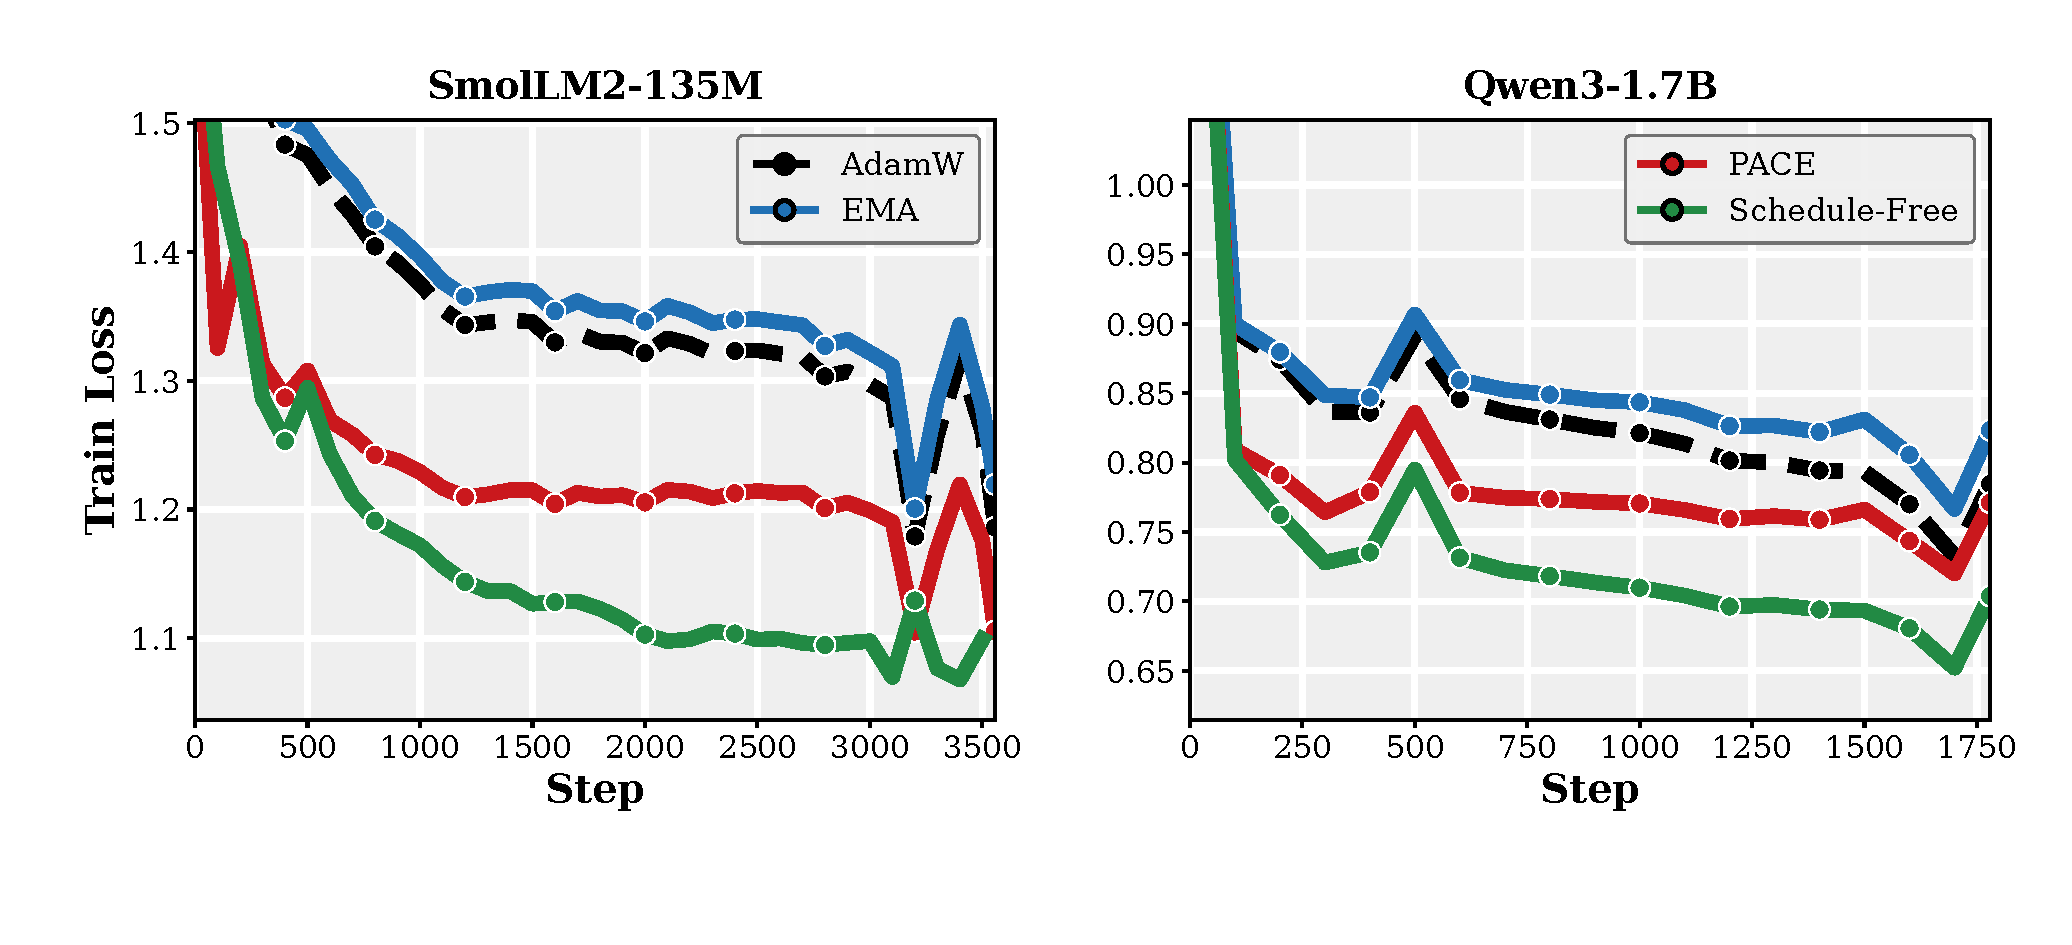
\includegraphics[width=0.667\textwidth]{figures/fig_appendix_train_curves.pdf}
  \caption{\textbf{Training-loss comparison of \pace\ to Schedule-Free \citep{defazio2024schedule}, AdamW, and EMA on fine-tuning.} Smoothed training loss on the same model selections as Fig.~\ref{fig:bema_sf}. Although \pace\ has higher training loss than Schedule-Free in this view, its validation loss is competitive in Fig.~\ref{fig:bema_sf}.}
  \label{fig:appendix_train_curves}
\end{figure}

\begin{figure}[ht]
  \centering
  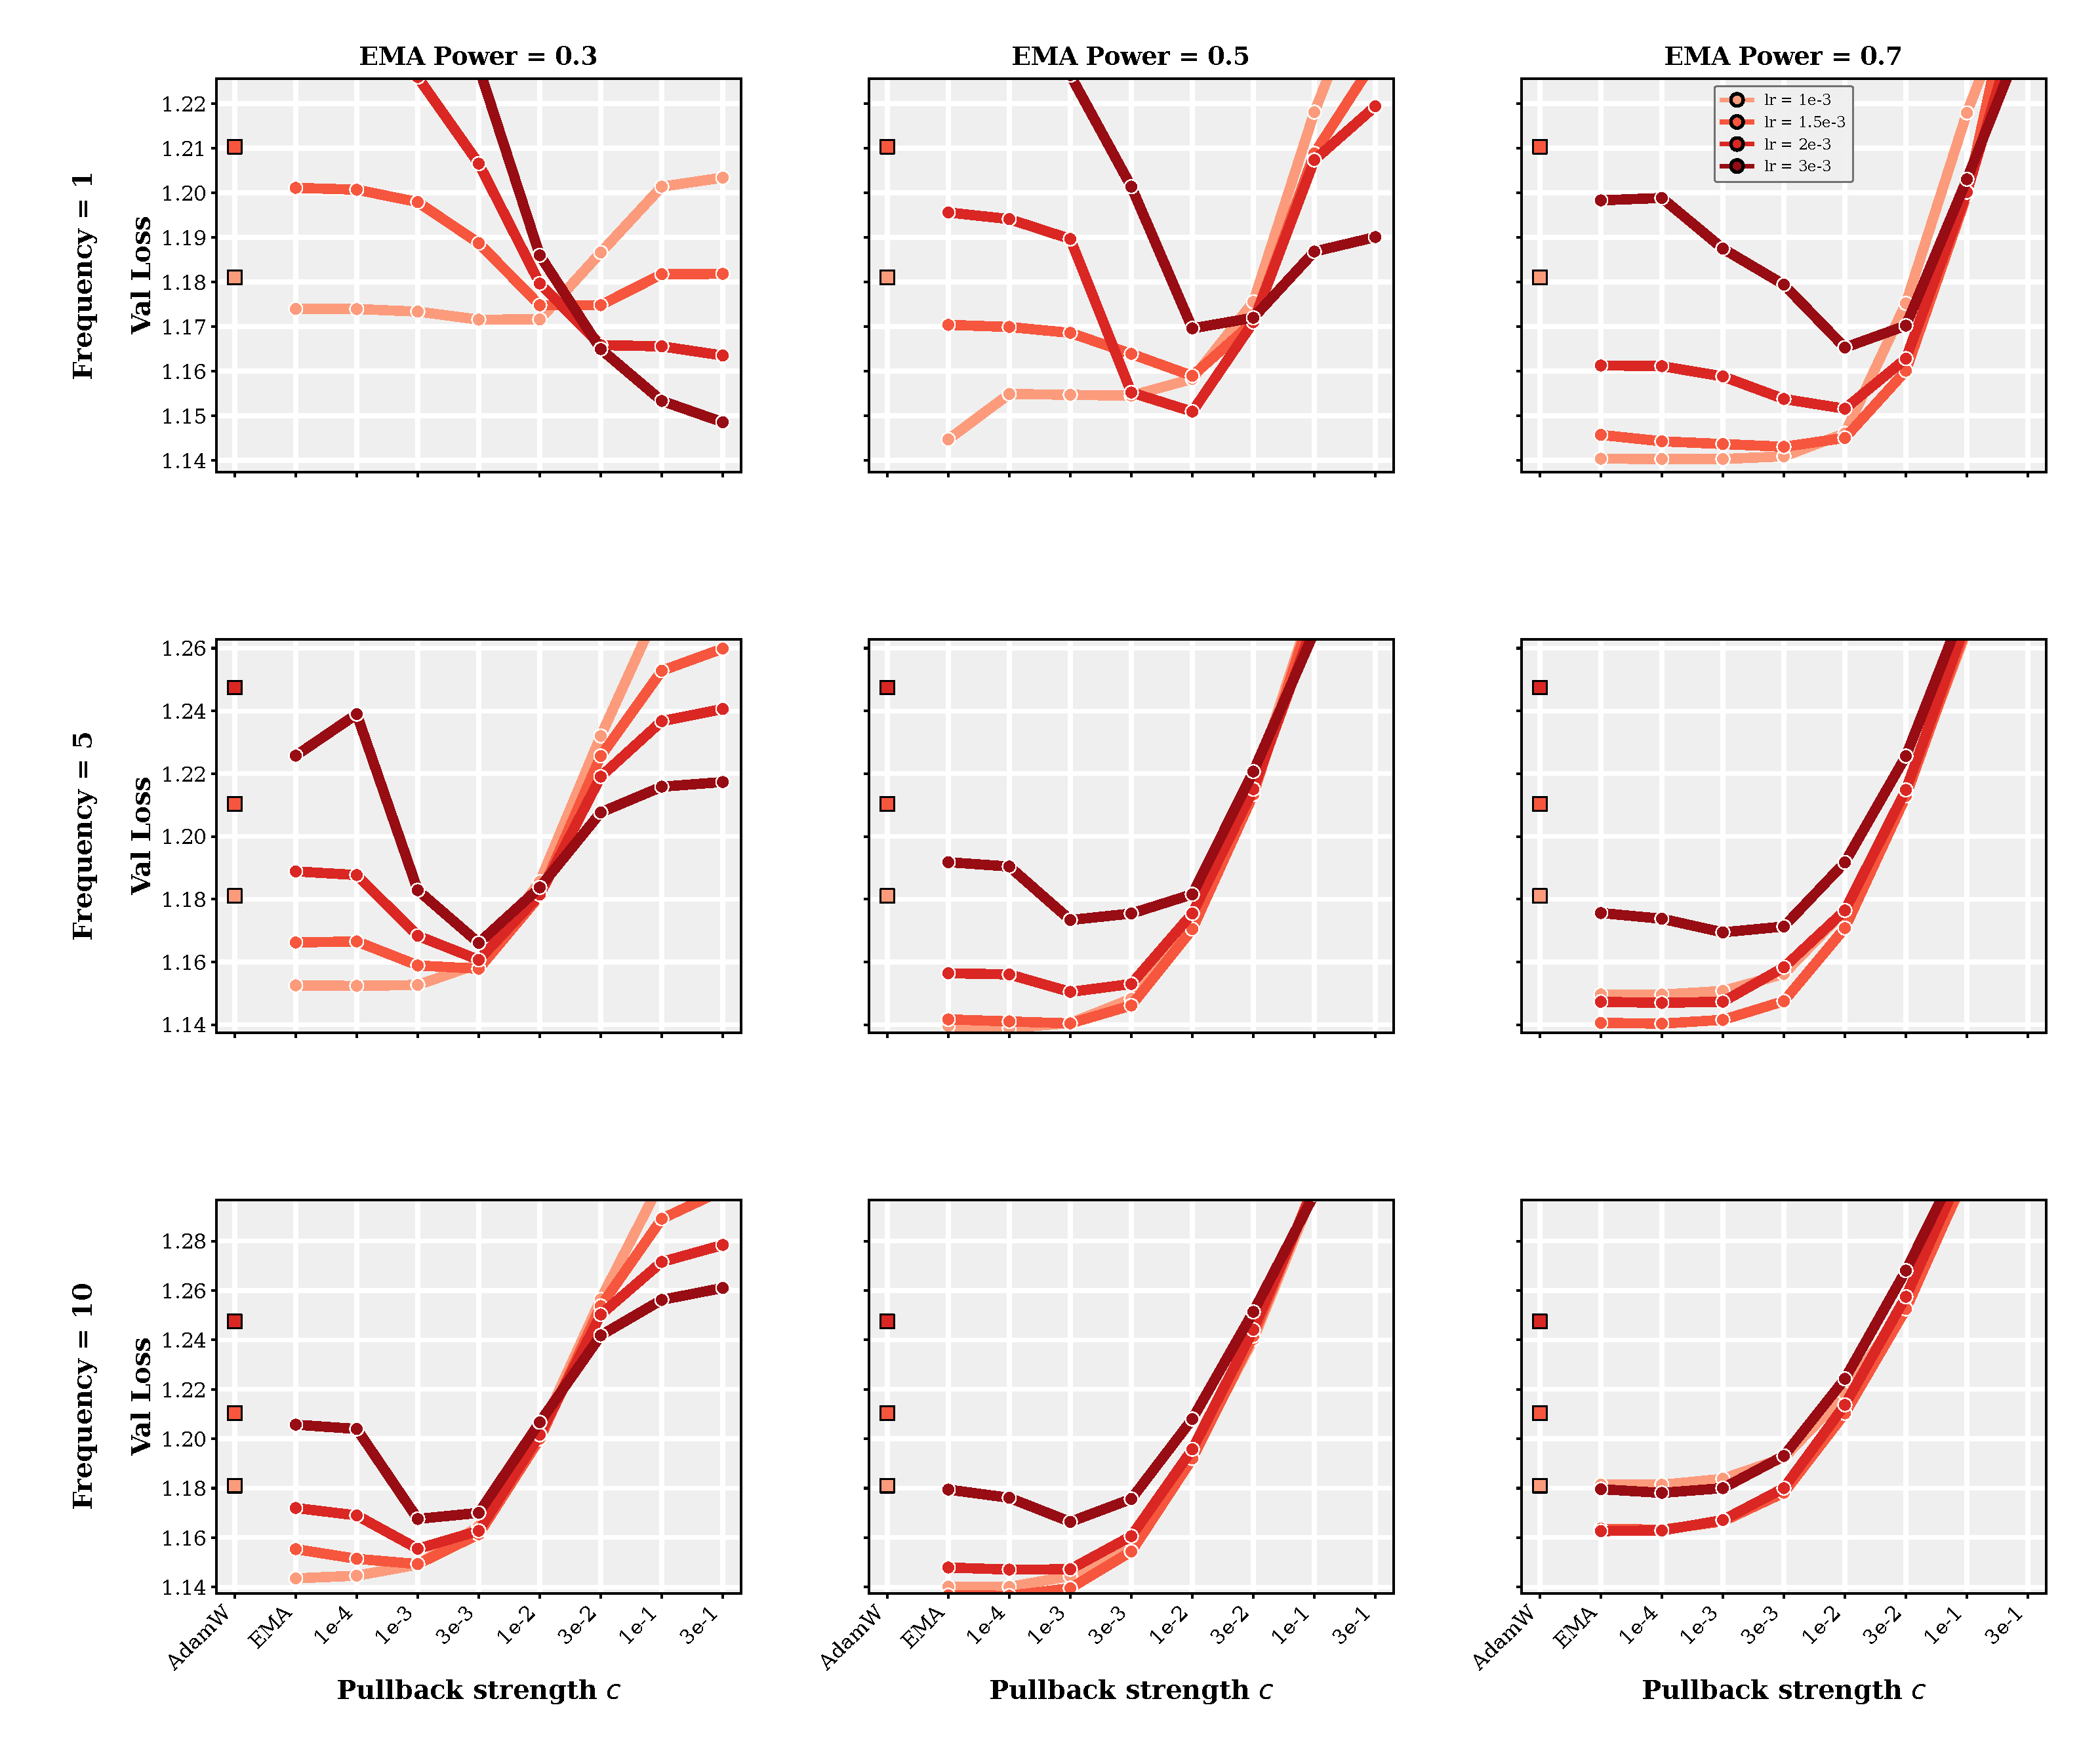
\includegraphics[width=\textwidth]{figures/fig_appendix_135m_full_grid.pdf}
  \caption{\textbf{Effect of update frequency, EMA power, and pullback strength.} Validation cross-entropy of SmolLM2-135M for different learning rates, pullback strengths, EMA powers, and update frequencies. Optimal pullback strength remains relatively robust to learning rate and update frequency, with improvement over the EMA baseline across a wide range of settings.}
  \label{fig:appendix_135m_full_grid}
\end{figure}

\begin{figure}[ht]
  \centering
  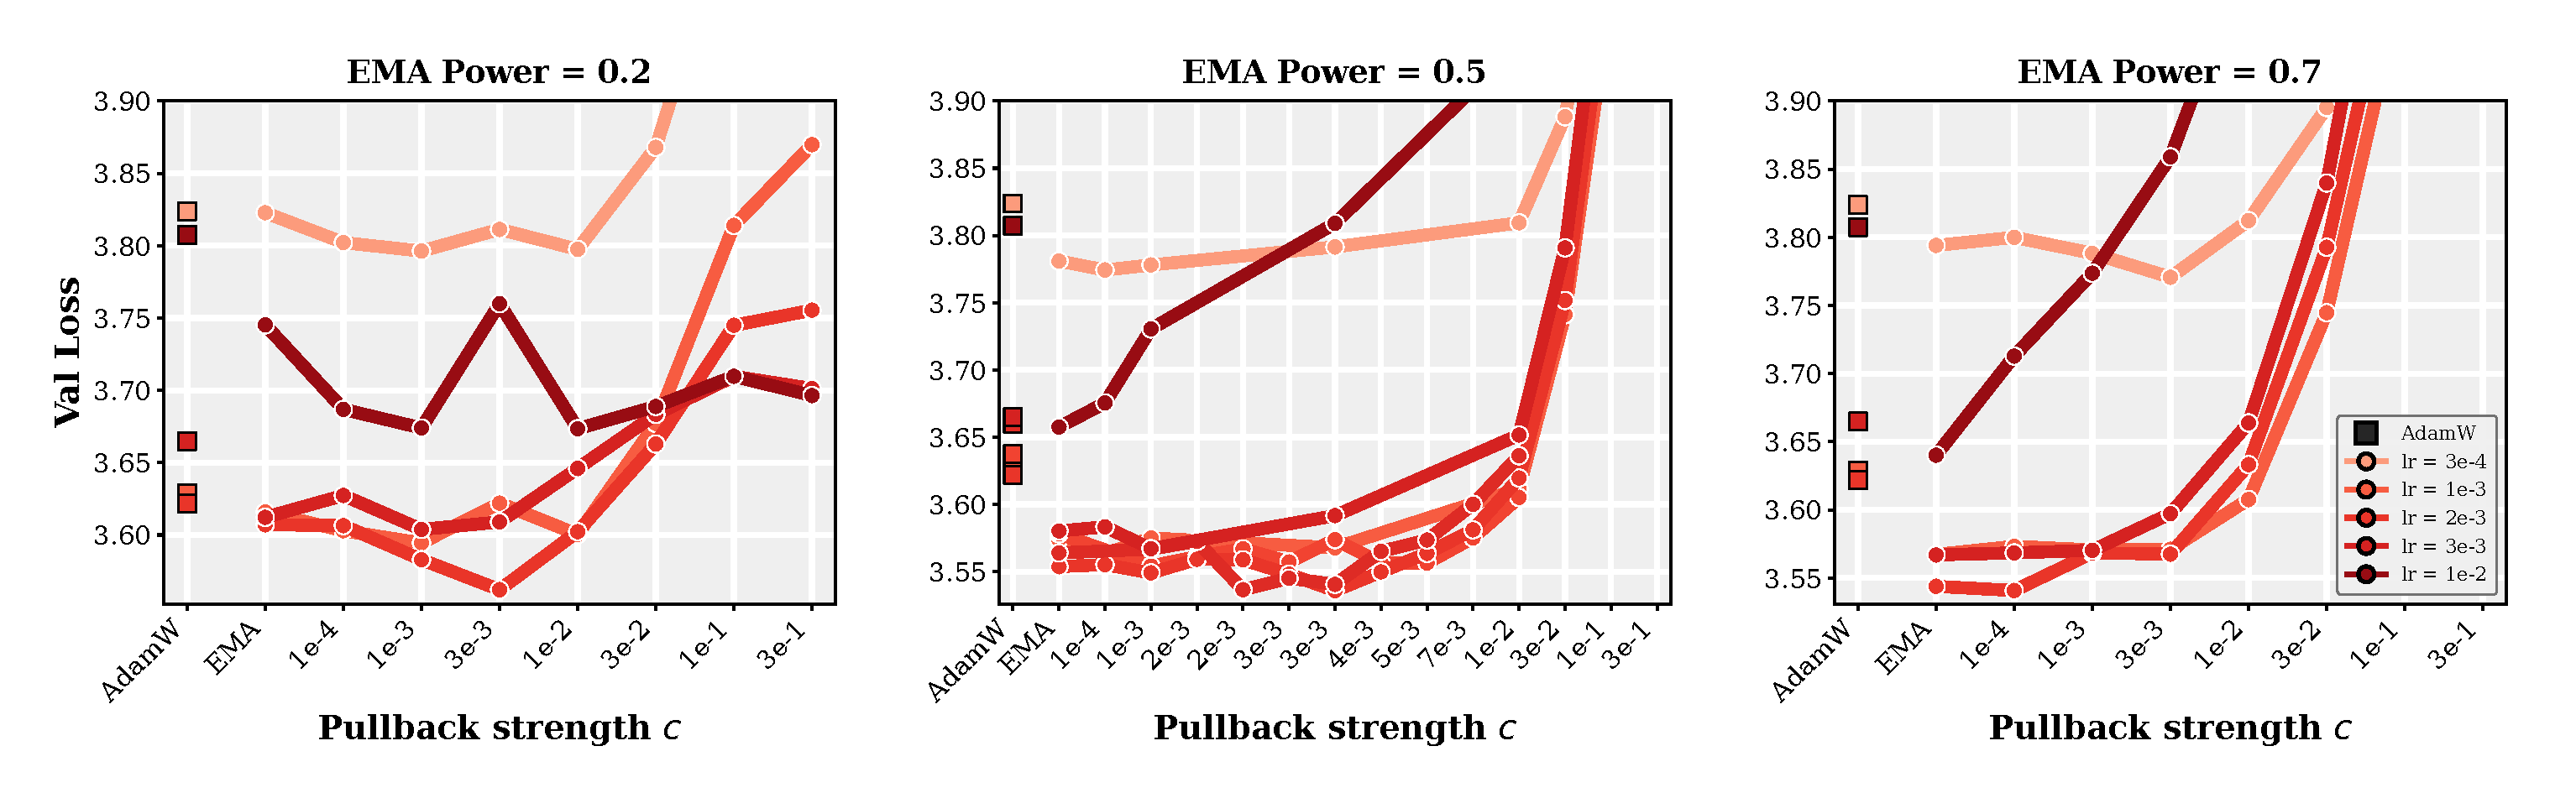
\includegraphics[width=\textwidth]{figures/fig_appendix_pretrain_kappa_sweep.pdf}
  \caption{\textbf{Effect of EMA power and pullback strength on pretraining.} Validation cross-entropy on GPT-2-124M trained on FineWeb for different learning rates, pullback strengths, and EMA powers. Optimal pullback strength remains robust, with improvement over the EMA baseline across a wide range of settings.}
  \label{fig:appendix_pretrain_kappa_sweep}
\end{figure}

\begin{figure}[ht]
  \centering
  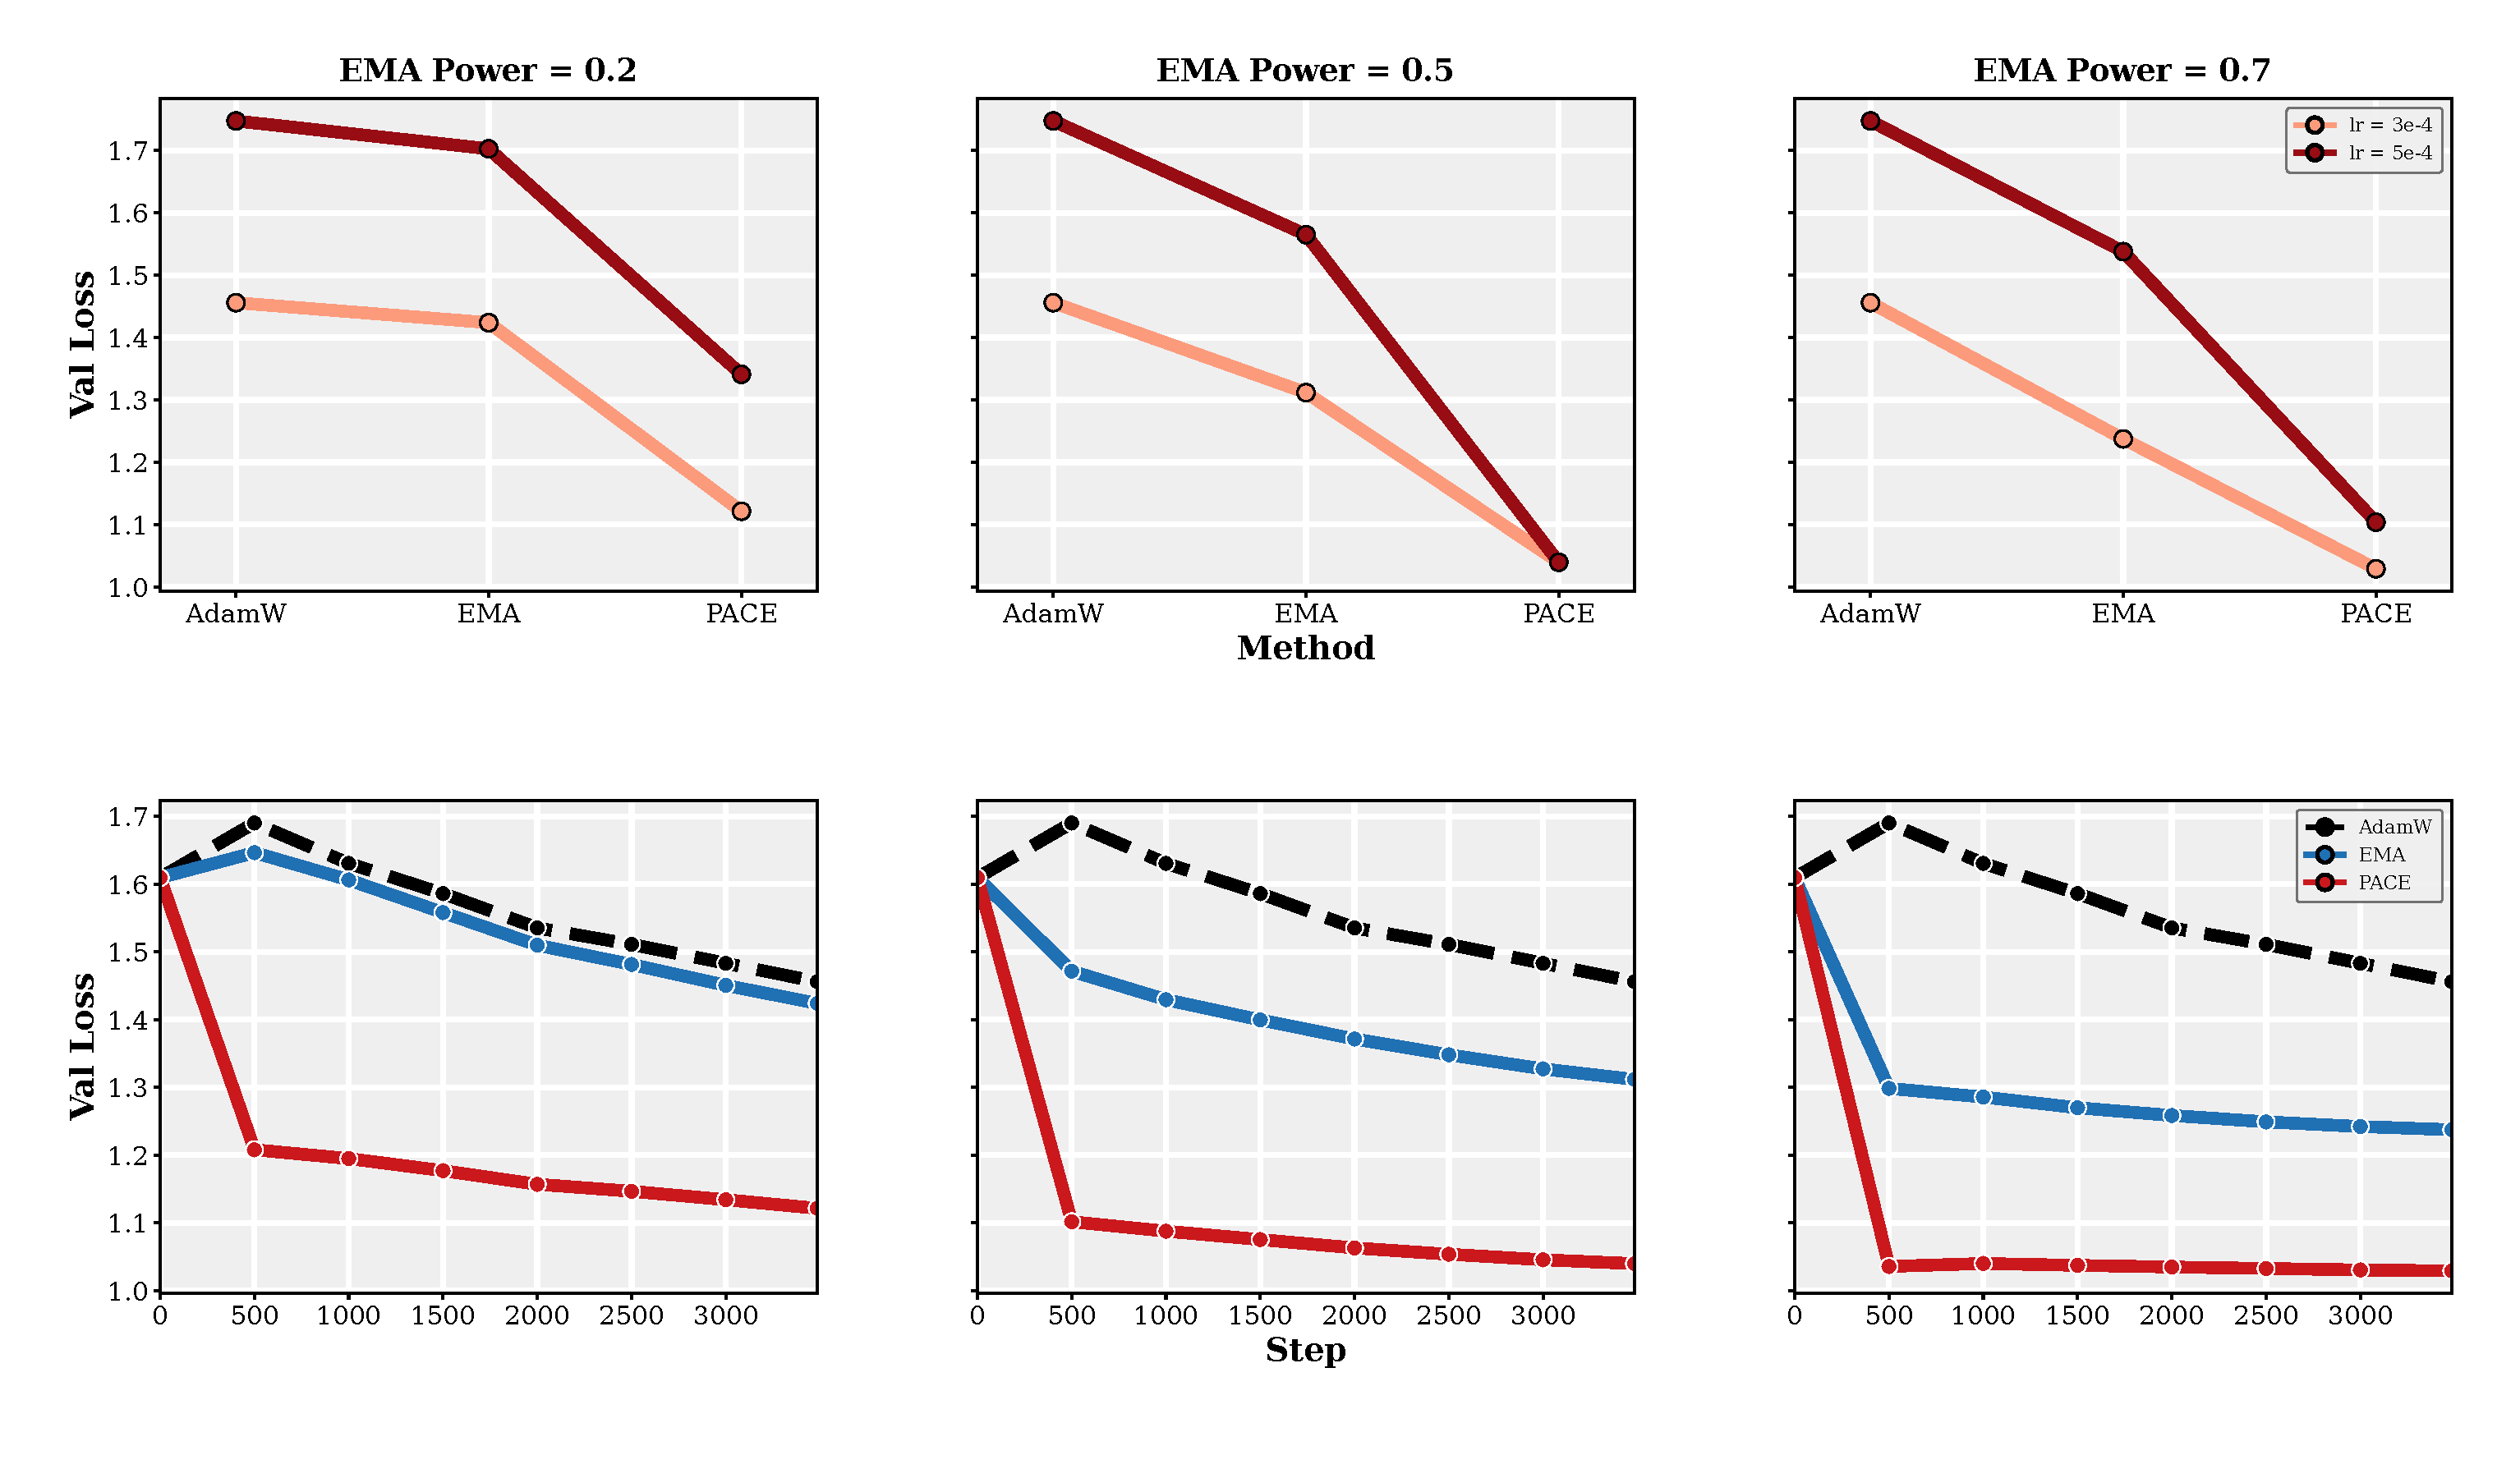
\includegraphics[width=\textwidth]{figures/fig_appendix_tulu_qwen.pdf}
  \captionof{figure}{\textbf{Effect of EMA power and pullback strength on Qwen3-1.7B Tulu-3 fine-tuning.} Validation cross-entropy across learning rates and EMA powers. \textbf{Top:} final validation loss for AdamW, EMA, and \pace. \textbf{Bottom:} validation trajectories at $\eta=3{\times}10^{-4}$. \pace\ improves over the matched AdamW and EMA baselines across the reported settings.}
  \label{fig:appendix_tulu_qwen}
\end{figure}

\begin{figure}[ht]
  \centering
  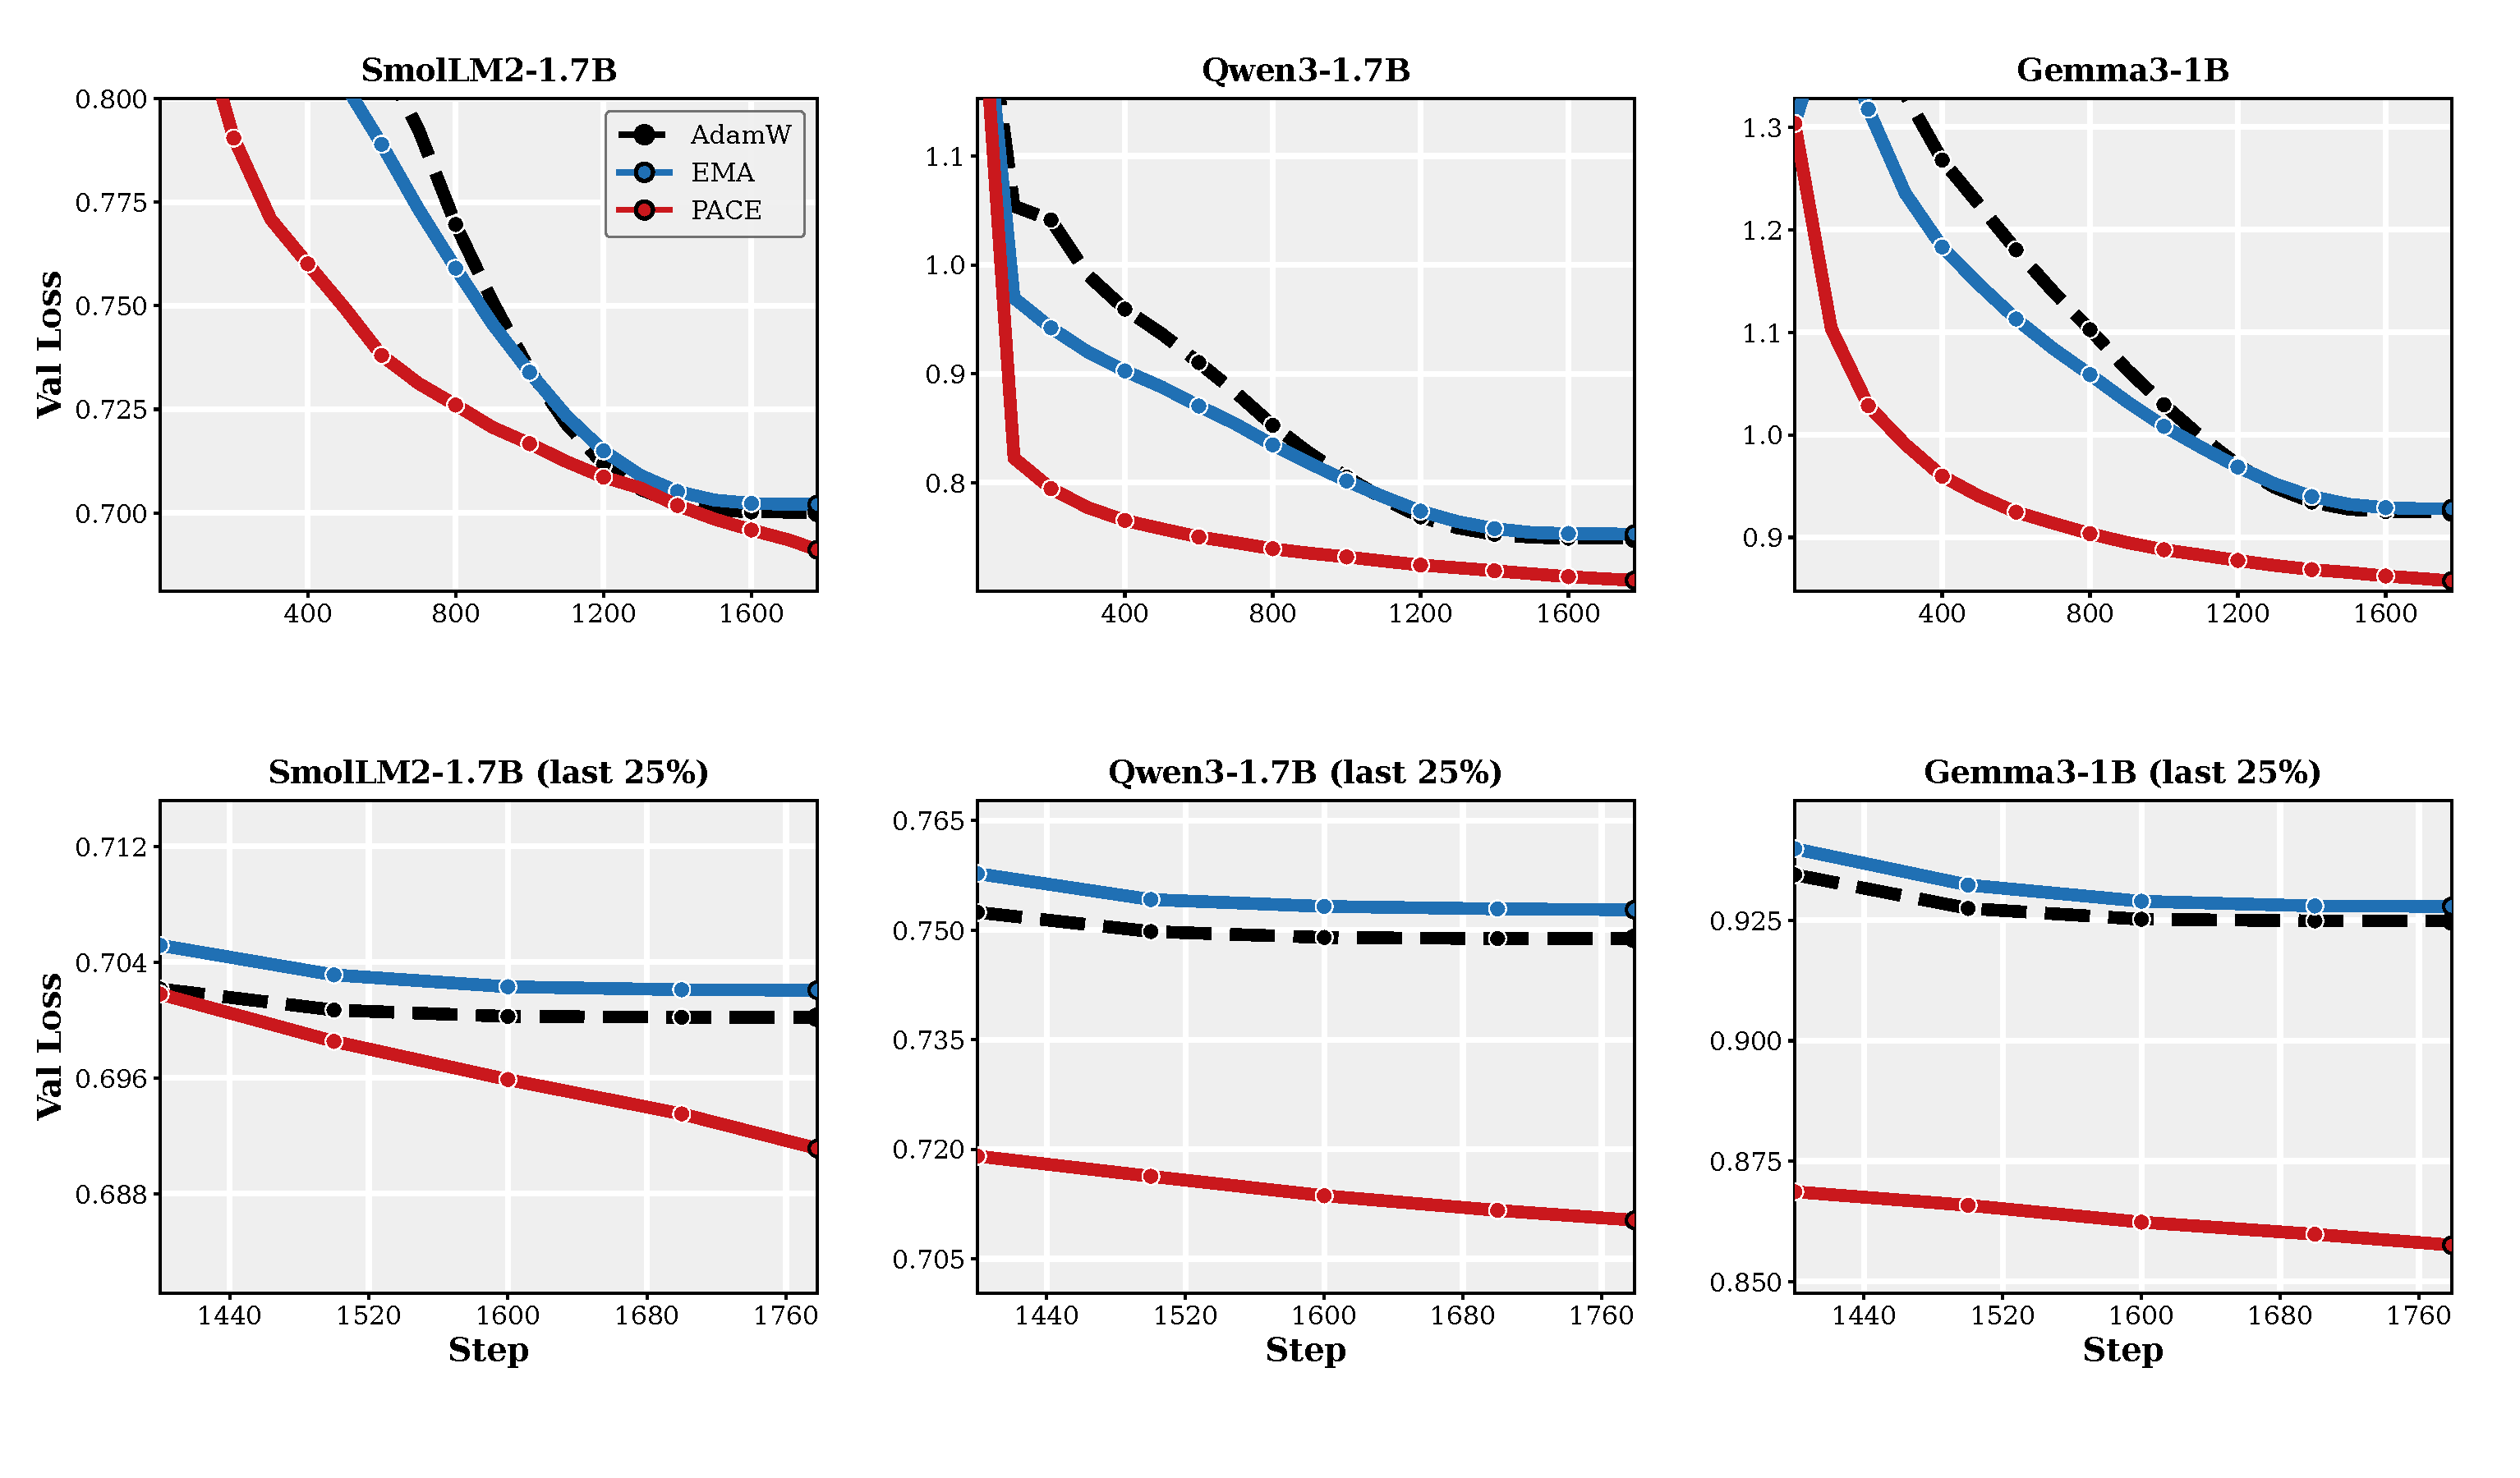
\includegraphics[width=\textwidth]{figures/fig_appendix_full_train_curves.pdf}
  \caption{\textbf{Last 25\% of the cross-entropy trajectories from Fig.~\ref{fig:train_curves}.} The top row shows the full validation trajectories, and the bottom row zooms into the final quarter of training. \pace\ shows a clear improvement on SmolLM2-1.7B, Qwen3-1.7B, and Gemma3-1B.}
  \label{fig:appendix_full_train_curves}
\end{figure}

\begin{figure}[ht]
  \centering
  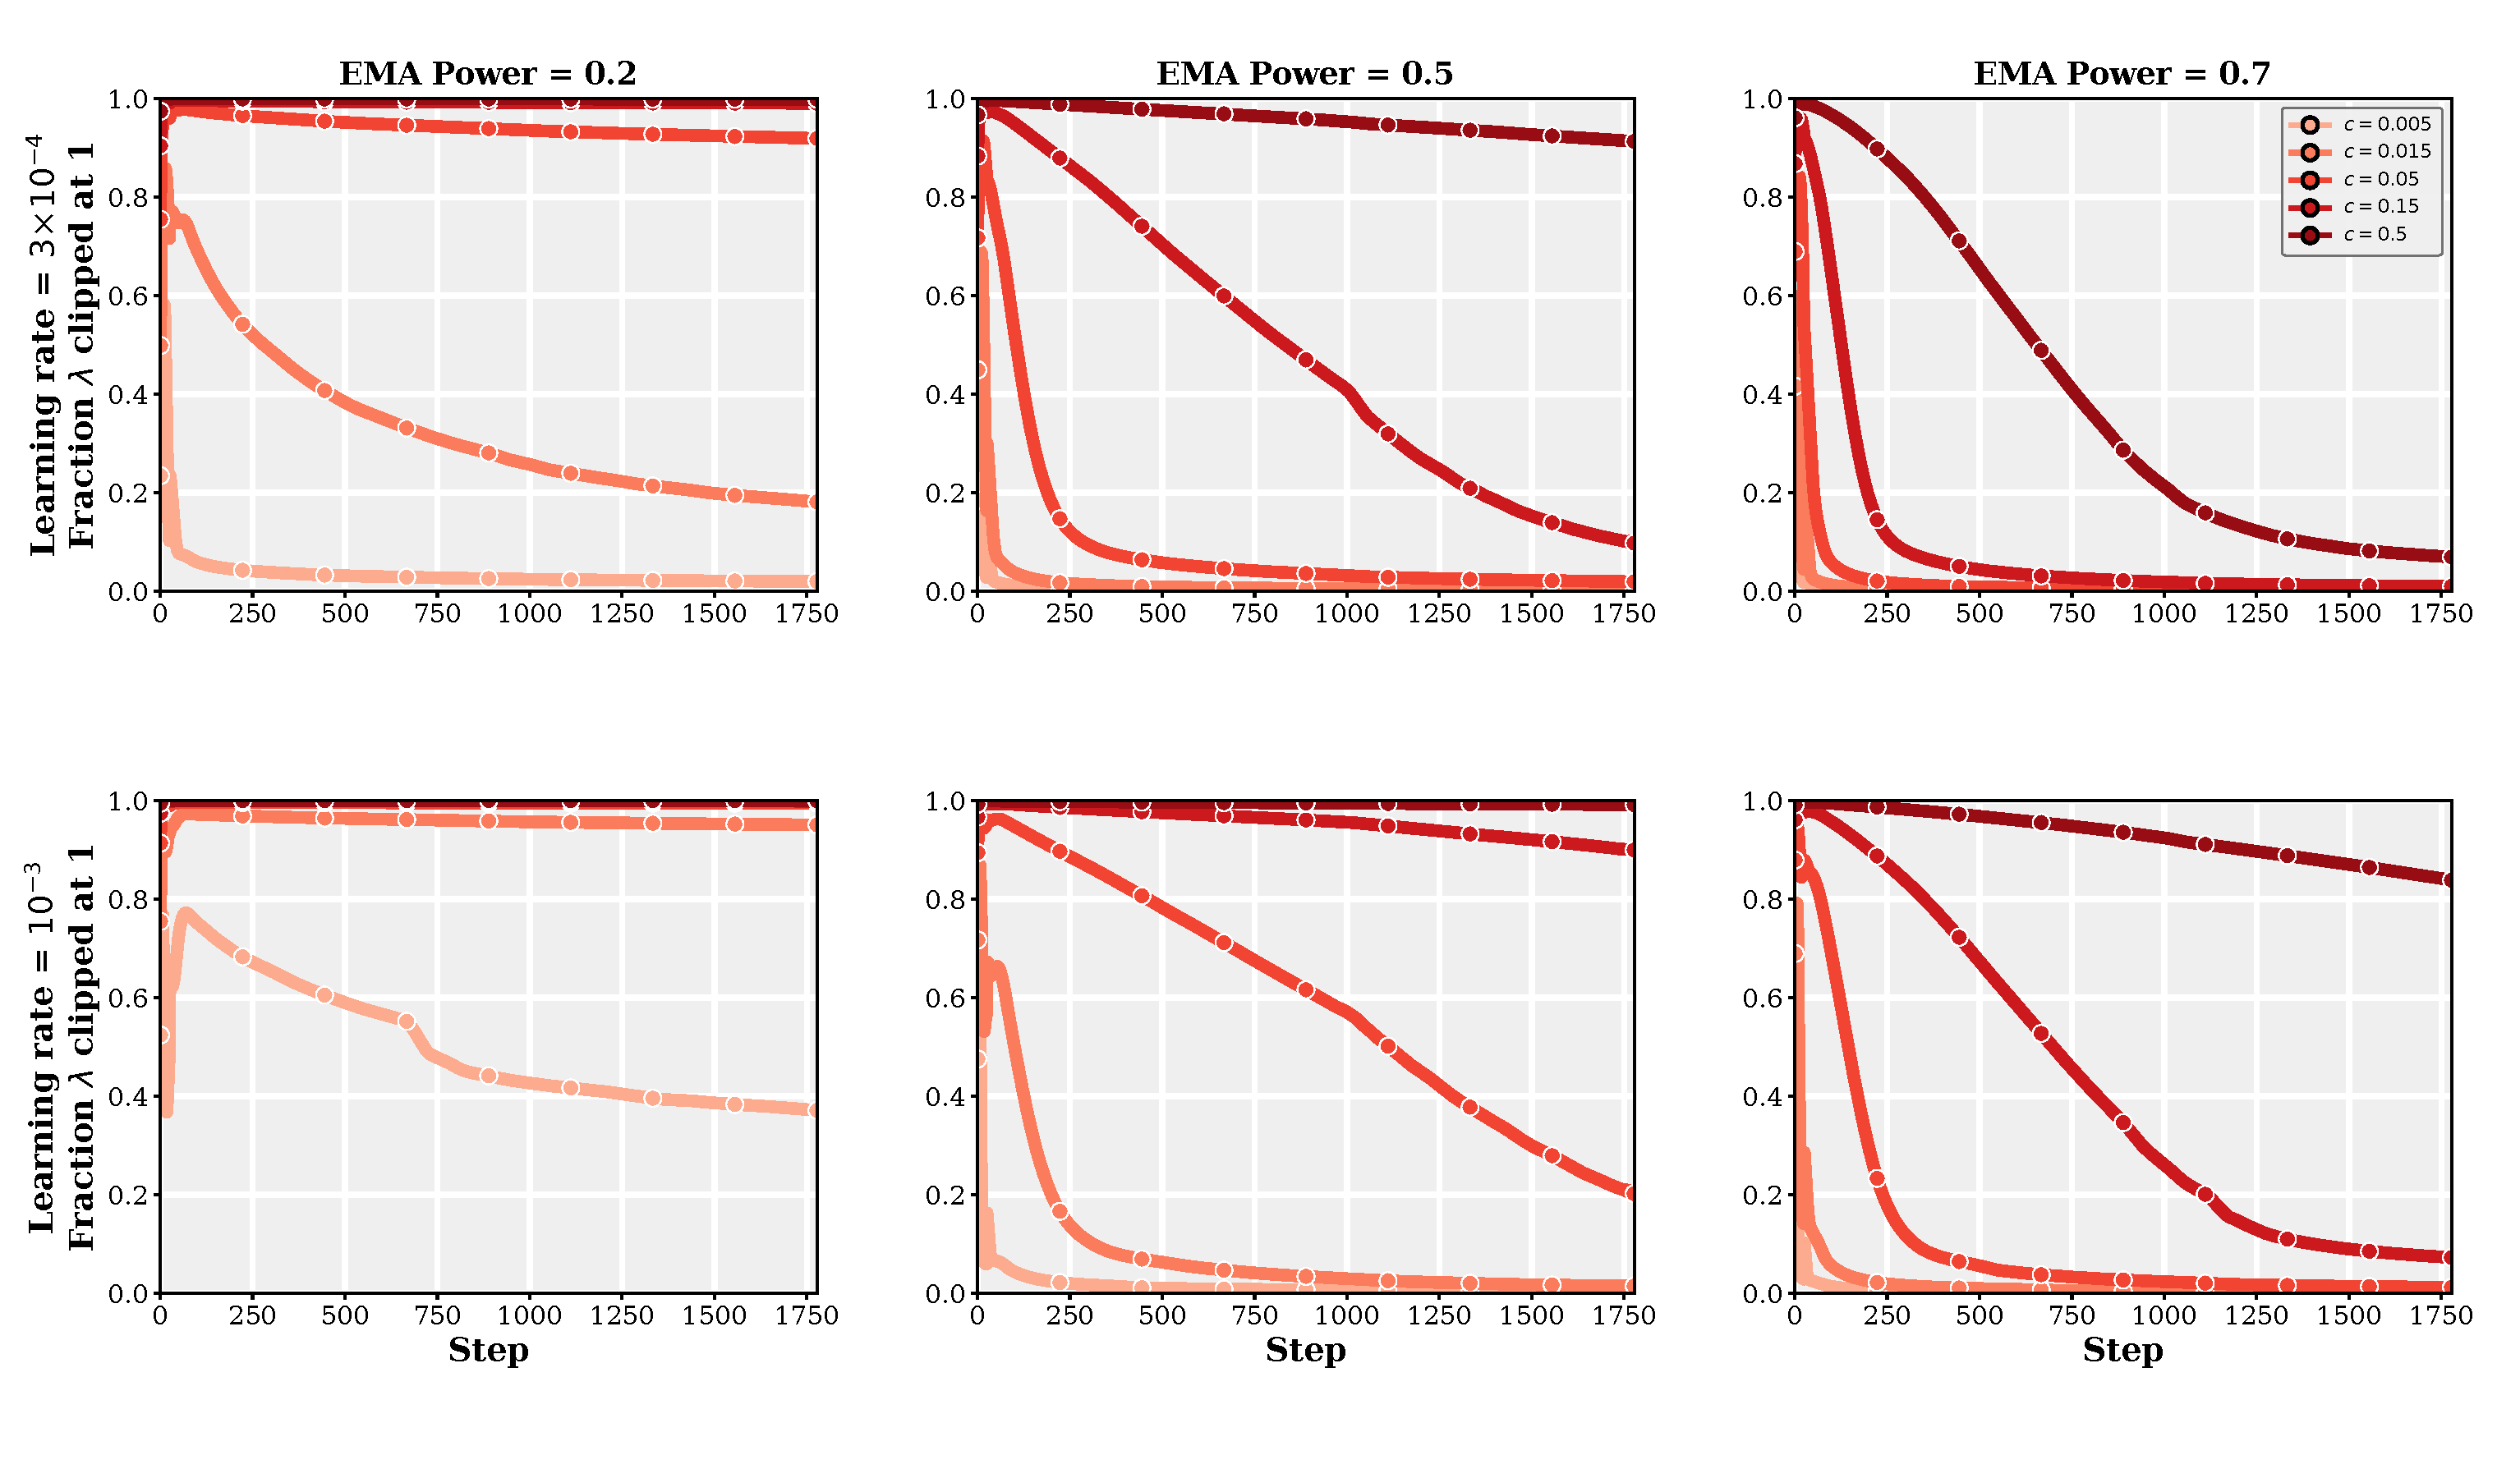
\includegraphics[width=\textwidth]{figures/fig_appendix_clip_frac.pdf}
  \caption{\textbf{Fraction of clipped updates over training.} Fraction of parameters with saturated pullback gain $\lambda_{t,i}=1$ on SmolLM2-1.7B, across learning rate, EMA power, and pullback strength. Saturation increases with pullback strength and is most pronounced for smaller EMA power.}
  \label{fig:appendix_clip_frac}
\end{figure}

\begin{figure}[ht]
  \centering
  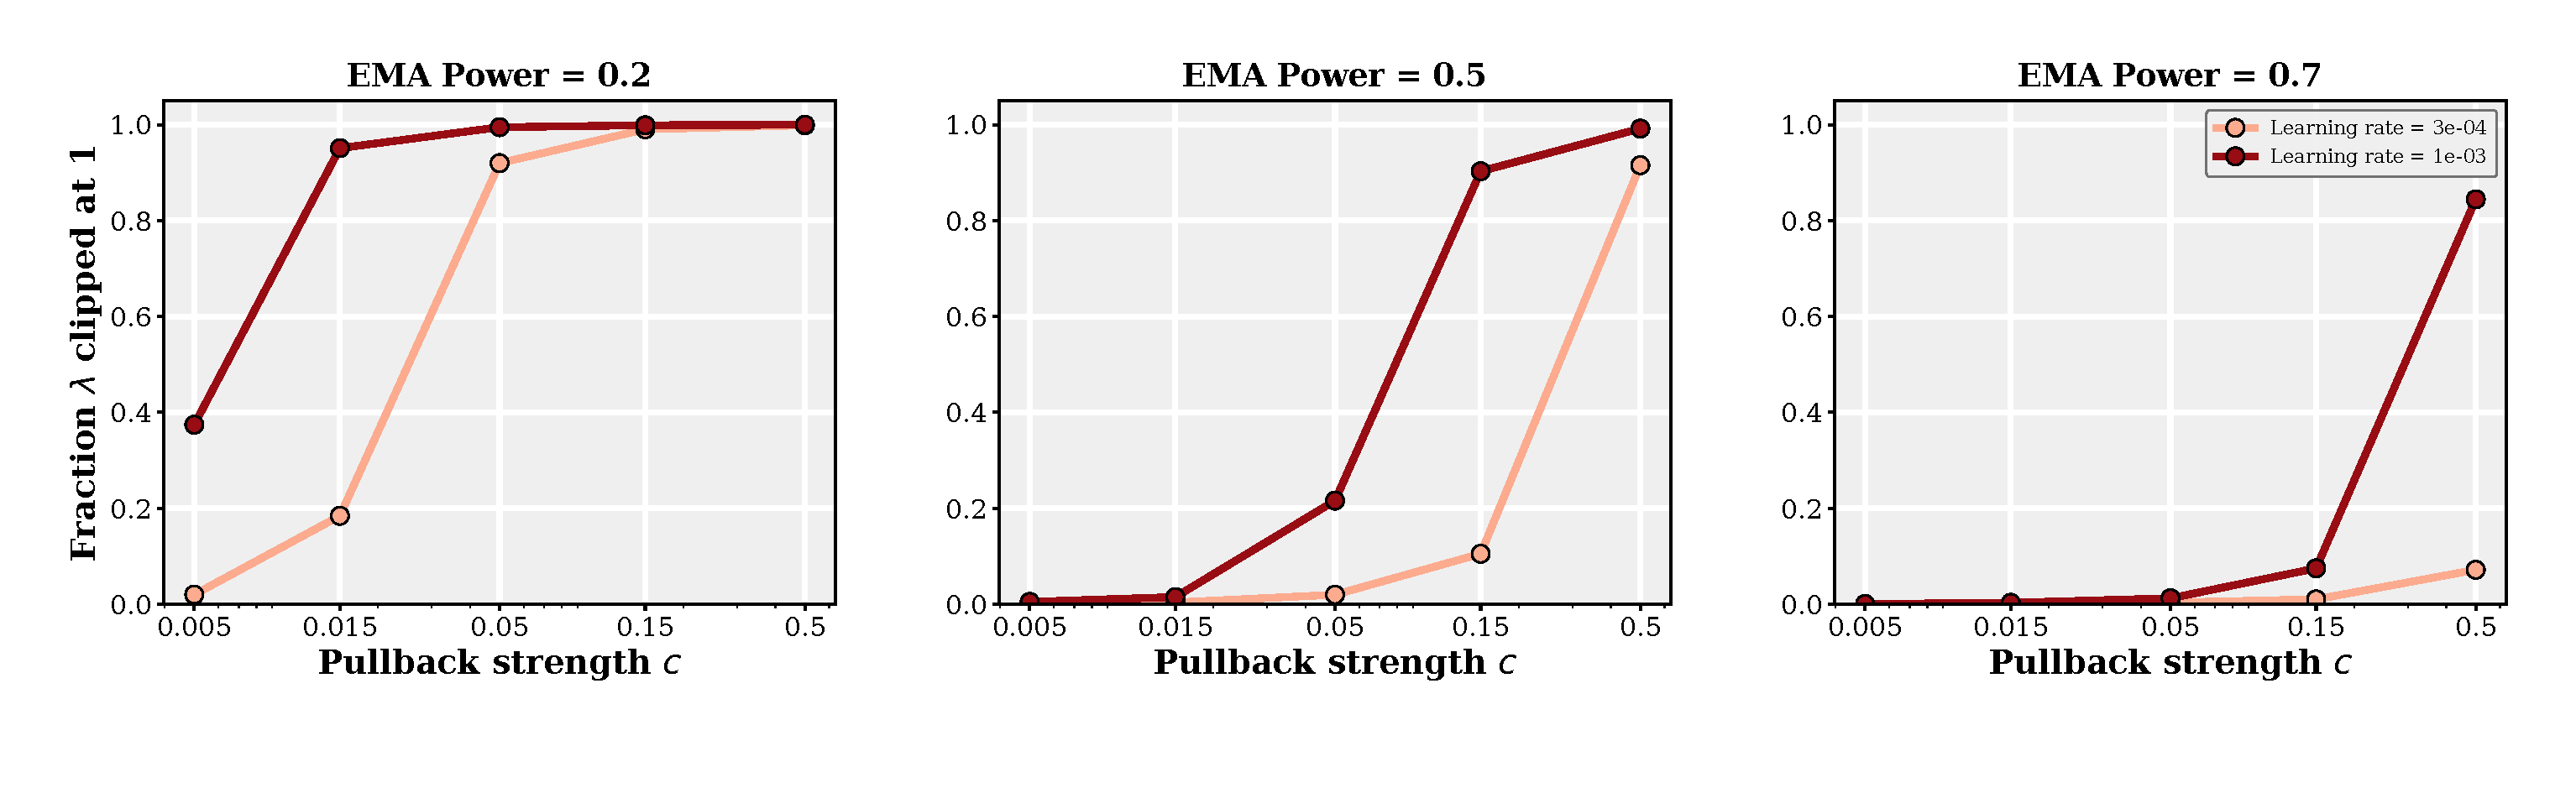
\includegraphics[width=\textwidth]{figures/fig_appendix_clip_frac_vs_c.pdf}
  \caption{\textbf{End-of-training fraction of clipped updates.} Fraction of parameters with saturated pullback gain $\lambda_{t,i}=1$ on SmolLM2-1.7B as a function of pullback strength and learning rate. Smaller EMA power reaches saturation at smaller pullback strengths.}
  \label{fig:appendix_clip_frac_vs_c}
\end{figure}

\begin{figure}[ht]
  \centering
  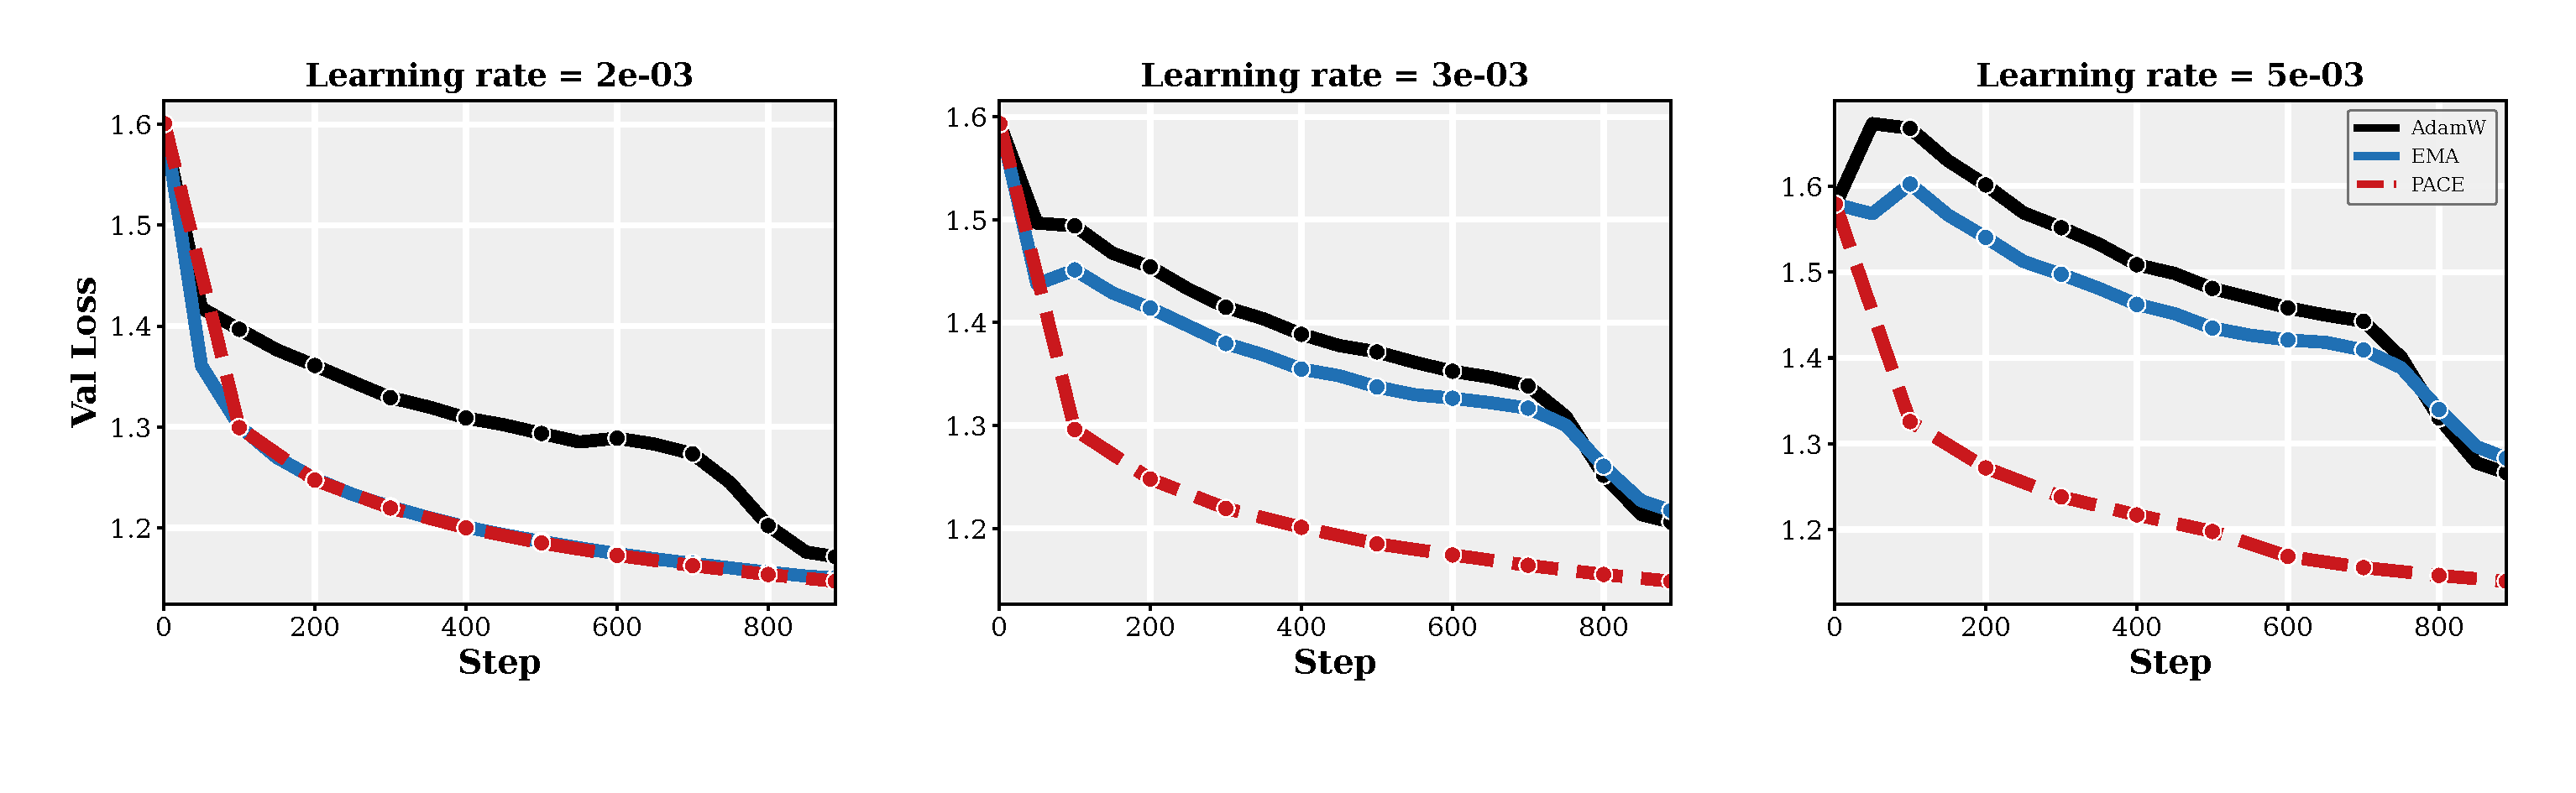
\includegraphics[width=\textwidth]{figures/fig_appendix_wsd_val_curves.pdf}
  \caption{\textbf{\pace\ against AdamW and EMA under fine-tuning.} Validation cross-entropy on SmolLM2-135M at three learning rates, with the baselines given their best decay schedule and \pace\ held at a constant learning rate. \pace\ ends below both baselines at every learning rate, and its margin over them grows sharply as the learning rate increases.}
  \label{fig:appendix_wsd_val_curves}
\end{figure}

